%%%%%%%%%%%%%%%%%%%%%%%%%%%%%%%%%%%%%%%%%%%%%%%%%%%%%%%%%%%%%%%%%%%%%%%%%%%%%%%%%%%%%%%%%%%%%%%%%%%
%%%%%%%%%%%%%%%%%%%%%%%%%%%%%%%%%%%%%%%%%%%%%%%%%%%%%%%%%%%%%%%%%%%%%%%%%%%%%%%%%%%%%%%%%%%%%%%%%%%
%%%%%%%%%%%%%%%%%%%%%%%%%%%%%%%%%%%%%%%%%%%%%%%%%%%%%%%%%%%%%%%%%%%%%%%%%%%%%%%%%%%%%%%%%%%%%%%%%%%
%%%%%%%%%%%%%%%%%%%%%%%%%%%%%%%%%%%%%%%%%%%%%%%%%%%%%%%%%%%%%%%%%%%%%%%%%%%%%%%%%%%%%%%%%%%%%%%%%%%

%\begin{figure}
%\centering
%\includegraphics[width=0.4\linewidth]
%{./img_diagramas/cabecita.pdf} 
%\caption{Representación esquemática de los sitios donde se encontraron diferencias 
%significativas en la comparación entre el porcentaje de épocas PE durante sueño MOR y NMOR, 
%para el grupo Control (ver texto)}
%\label{cabecita}
%\end{figure}

\chapter{Resultados}

\section{Estacionariedad en épocas pequeñas}

Una práctica común en el análisis de señales electrofisiológicas es el suponer que una serie de 
tiempo \textit{suficientemente} corta pueda considerarse estacionaria, cuando menos en el sentido
débil; anteriormente se ha señalado que se trata de un efecto de muestras pequeñas \cite{Melard89},
y paralelamente se han incorporado a los diseños experimentales motivos para mantener este supuesto
\cite{Kaiser00}.

Un análisis necesario en este trabajo es probar --en un sentido estadístico-- dicha hipótesis, para 
lo cual se ha adaptado la metodología particular de McEwen \cite{McEwen75} a los datos y técnicas 
presentados previamente: los registros se fragmentaron en épocas de diferentes tamaños, cada una de 
las cuales fue clasificada como estacionaria o no-estacionaria usando la prueba de PSR, y 
posteriormente se calculó el porcentaje de épocas estacionarias con respecto al total de épocas
para cada tamaño de época. 

La información obtenida representa, de manera normalizada, cómo la ocurrencia de épocas 
estacionarias depende de la longitud de las mismas; los tamaños de época se han elegido de la forma 
$30\times 2^{n}$ segundos, para poder considerar múltiplos y submúltiplos del tamaño de época
recomendado por la AASM (30 segundos).
En la figura \ref{cabeza_repoio} se muestra un ejemplo de estos datos, mientras que en el anexo E
se incluyen gráficos para todos los sujetos.


\begin{figure}
\centering
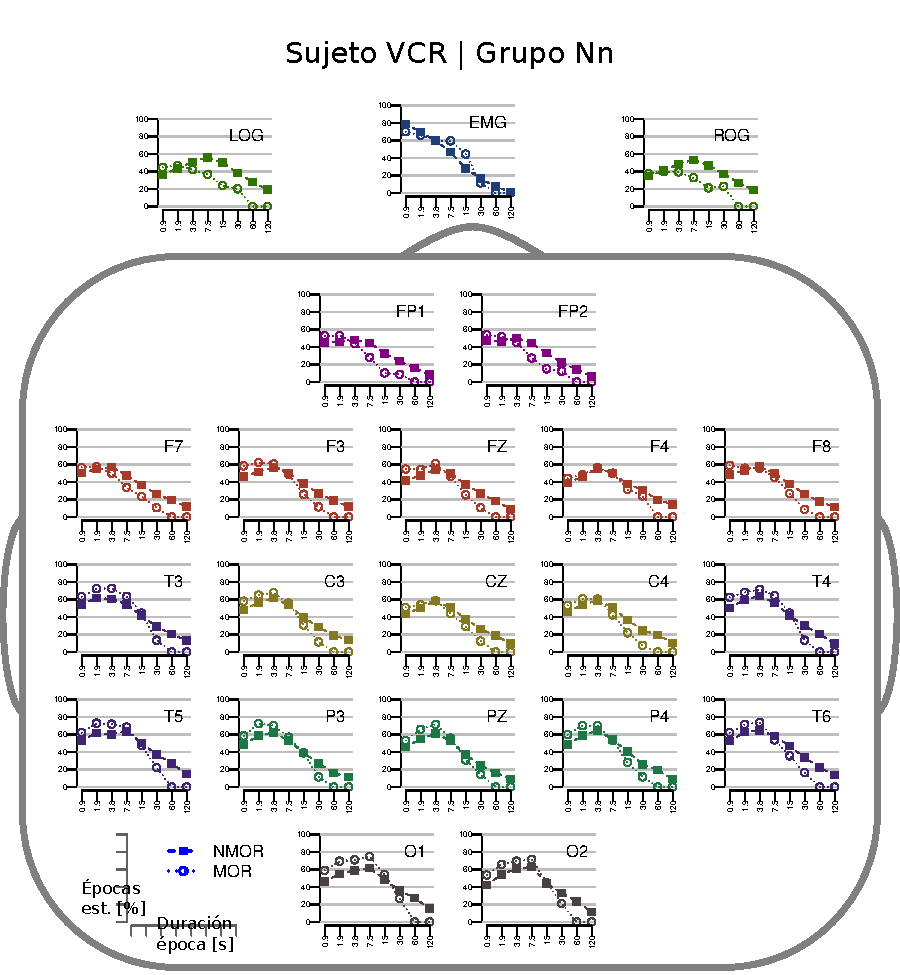
\includegraphics[width=.9\linewidth]{./img_resultados/cabeza_VCR.pdf}
\caption{Porcentajes de épocas estacionarias}
\label{cabeza_repoio}
\end{figure}

\section{Estacionariedad en sueño MOR}

En busca de una interpretación significativa de la estacionariedad débil, desde la fisiología del
sueño, se comparó si en sueño MOR era más frecuente la estacionariedad que en otras etapas de 
sueño, para lo cual se usó la prueba $\chi^{2}$ para proporciones\footnote{Implementada en R como 
\texttt{prop.test}} sobre las épocas (de 30 segundos) estacionarias en MOR y NMOR.
%
La diferencias encontradas no mostraron patrones consistentes claros entre los sujetos salvo por 
los canales LOG y ROG ($p<0.05$), que presentan proporciones mayores de épocas estacionarias 
durante sueño MOR (ver figura \ref{cabecitas_munchas}). Esto puede ser explicado por los 
movimientos oculares rápidos, característicos de dicha etapa de sueño.
%

\begin{figure}
\centering
\begin{tabular}{c}
\begin{tabular}{ccccc}
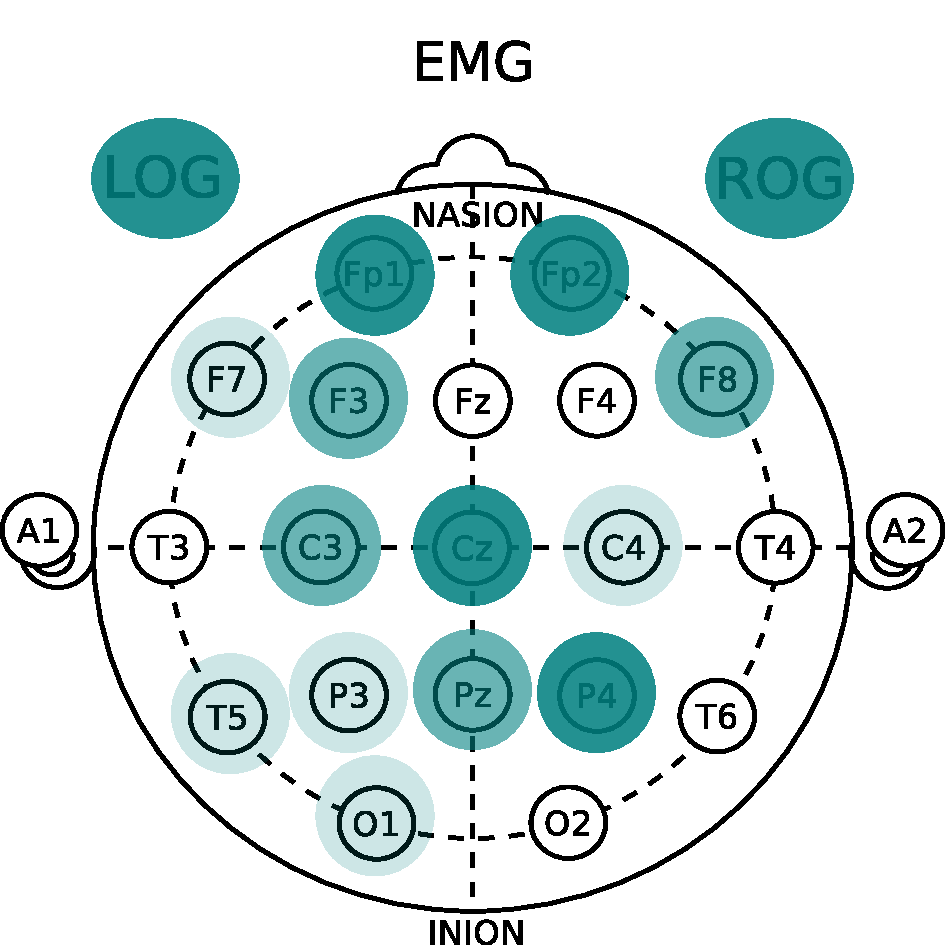
\includegraphics[width=0.15\textwidth]{./img_diagramas/cabecita_VCR.pdf} &
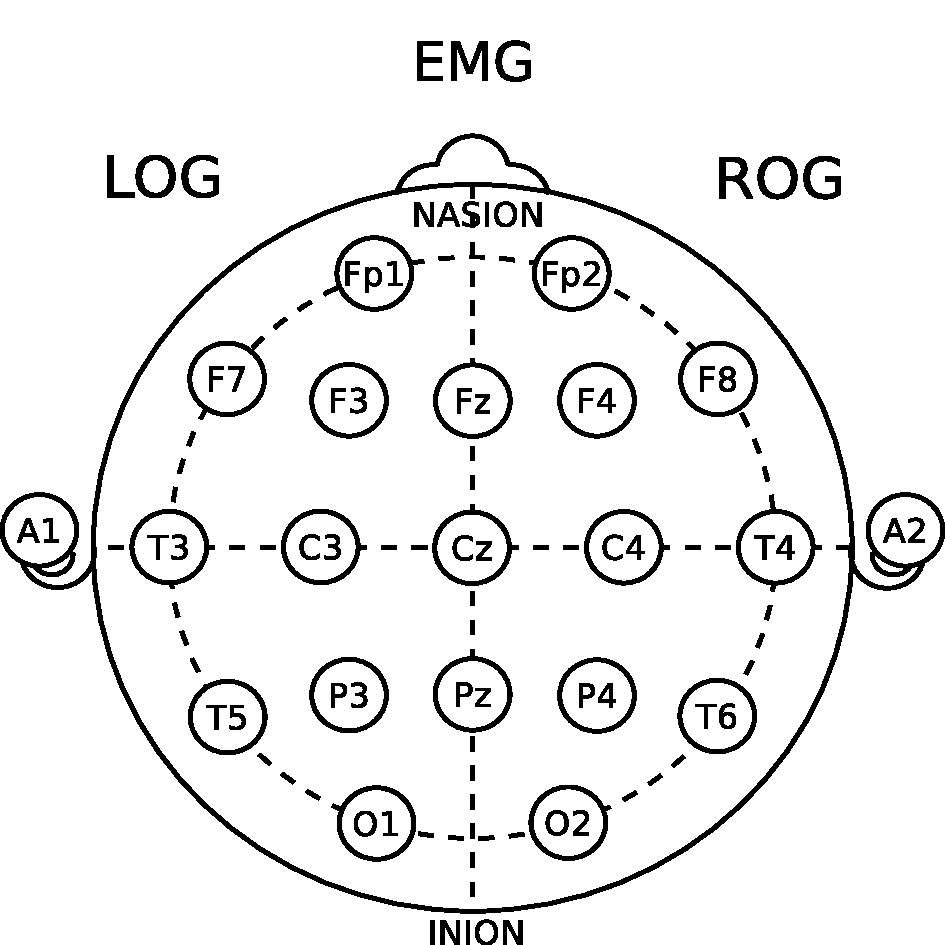
\includegraphics[width=0.15\textwidth]{./img_diagramas/cabecita_MJH.pdf} &
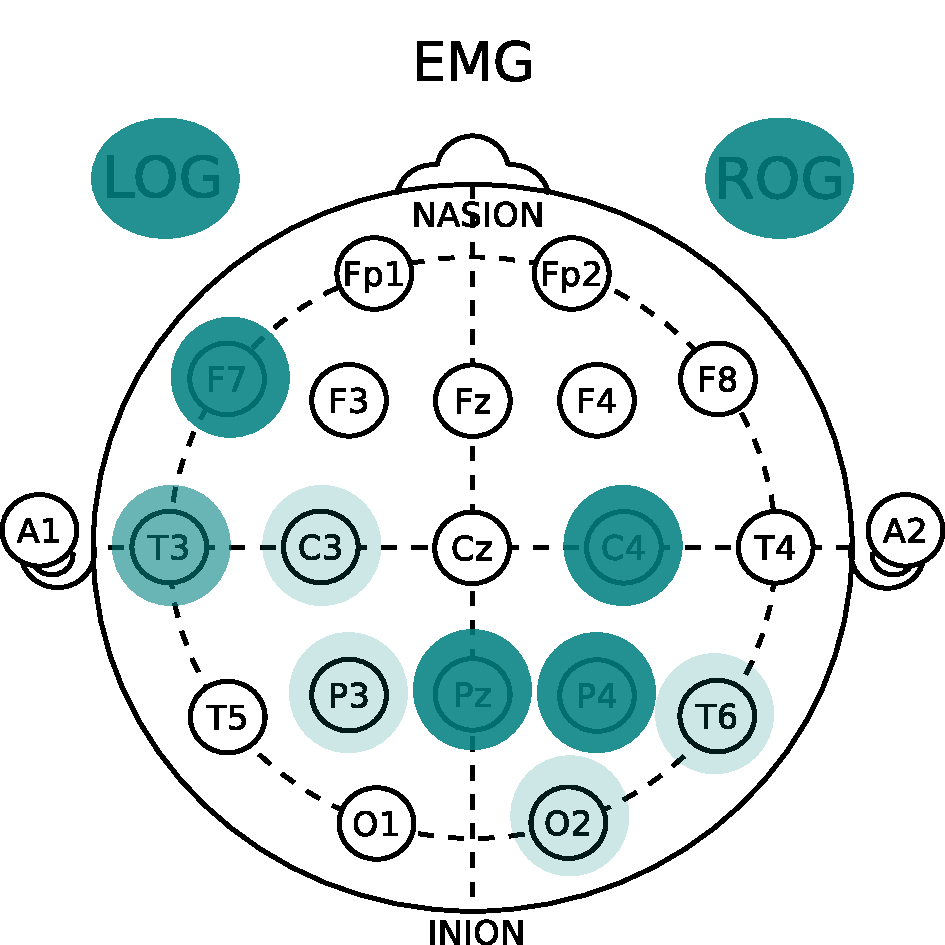
\includegraphics[width=0.15\textwidth]{./img_diagramas/cabecita_JAE.pdf} &
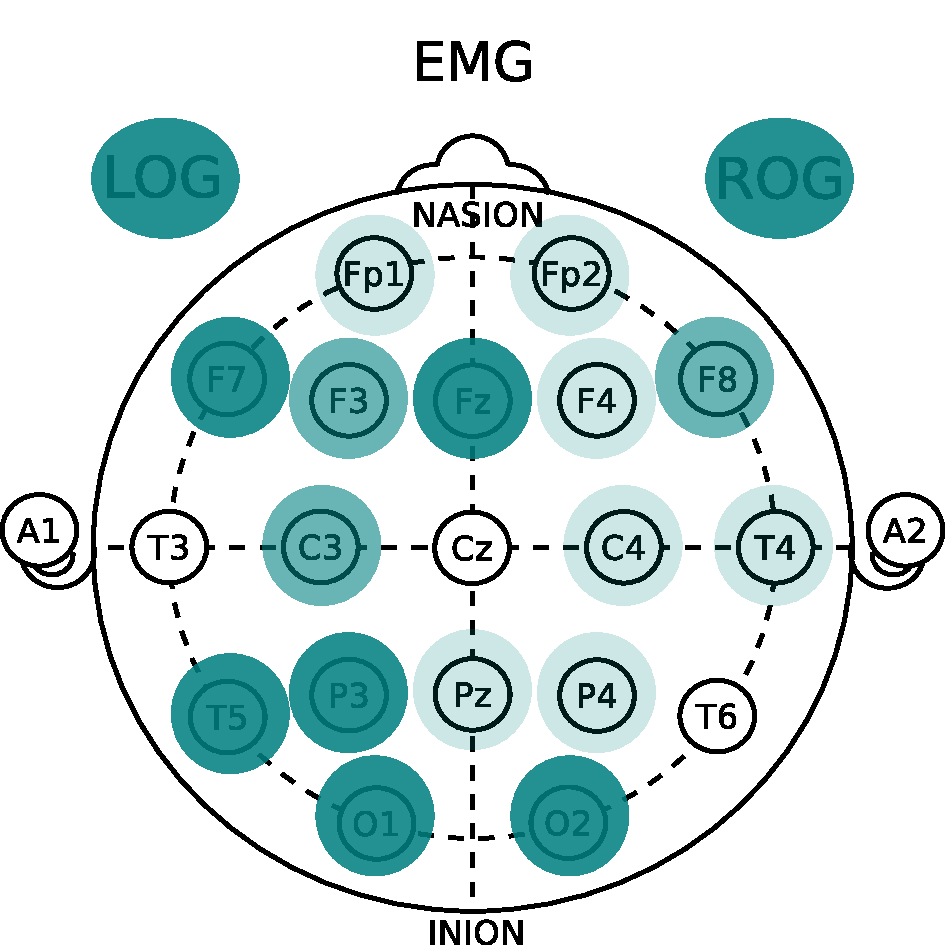
\includegraphics[width=0.15\textwidth]{./img_diagramas/cabecita_GHA.pdf} &
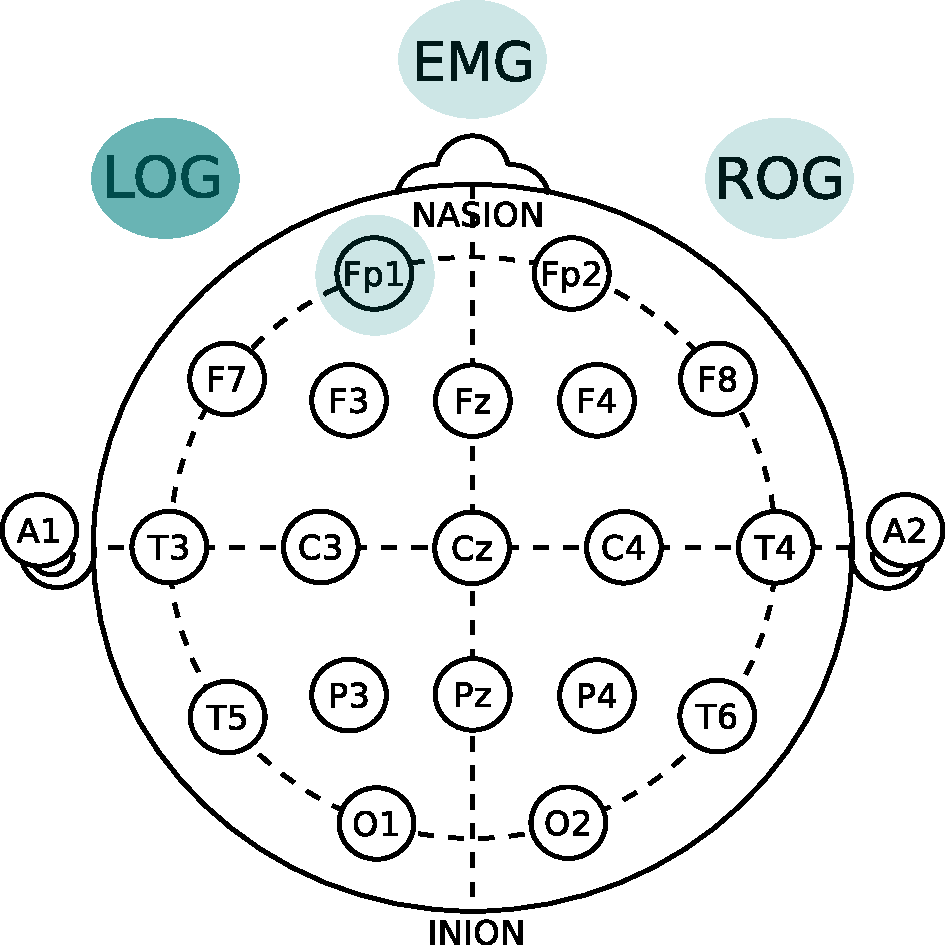
\includegraphics[width=0.15\textwidth]{./img_diagramas/cabecita_MFGR.pdf} \\
VCR & MJH & JAE & GHA & MFGR
\end{tabular}
\\
\begin{tabular}{cccc}
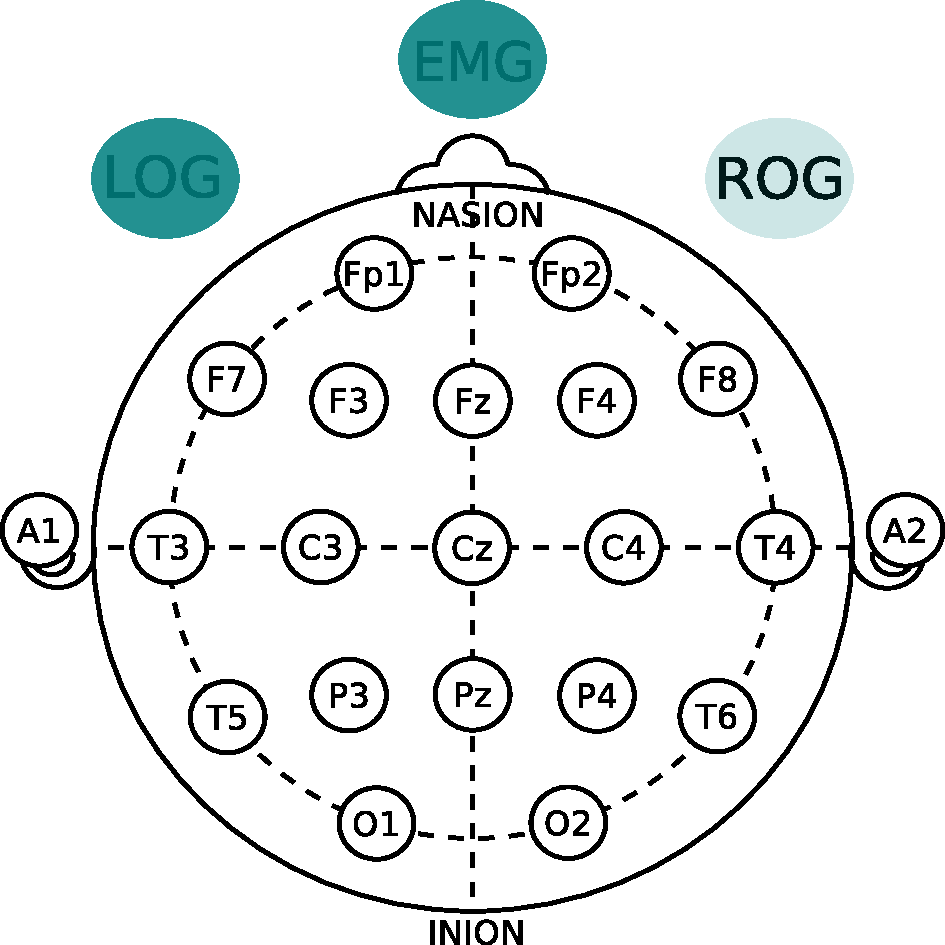
\includegraphics[width=0.15\textwidth]{./img_diagramas/cabecita_CLO.pdf} &
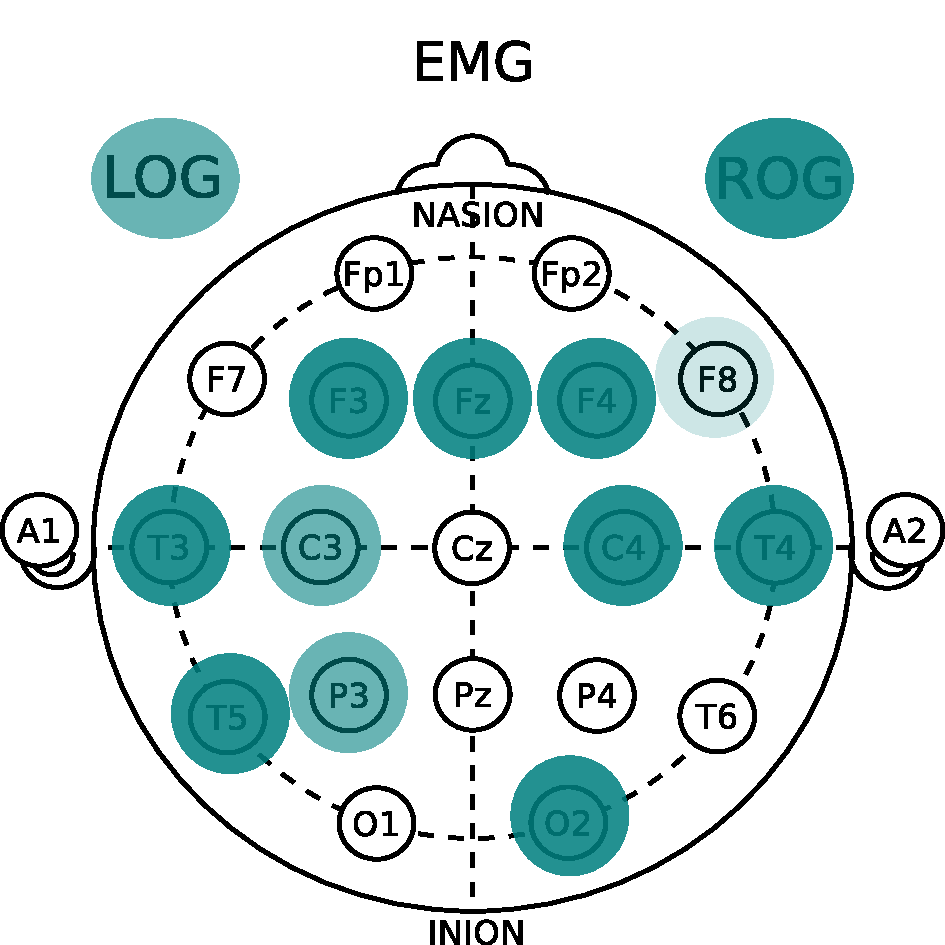
\includegraphics[width=0.15\textwidth]{./img_diagramas/cabecita_RLO.pdf} &
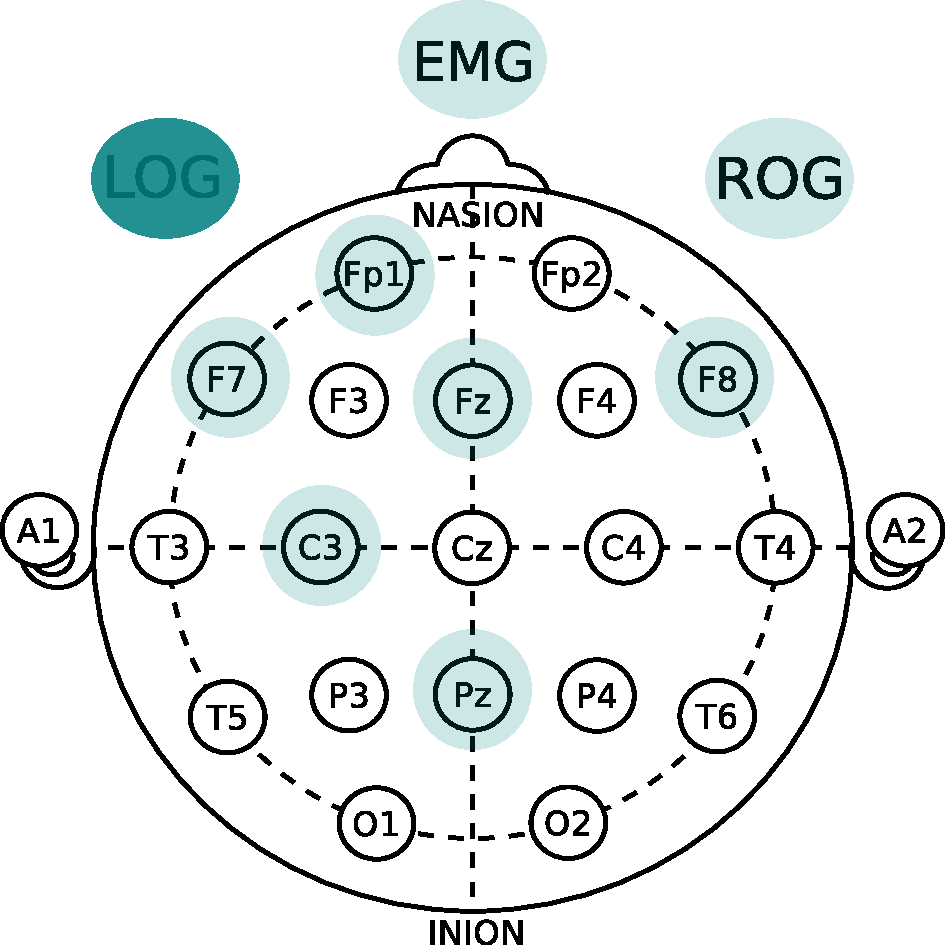
\includegraphics[width=0.15\textwidth]{./img_diagramas/cabecita_RRU.pdf} &
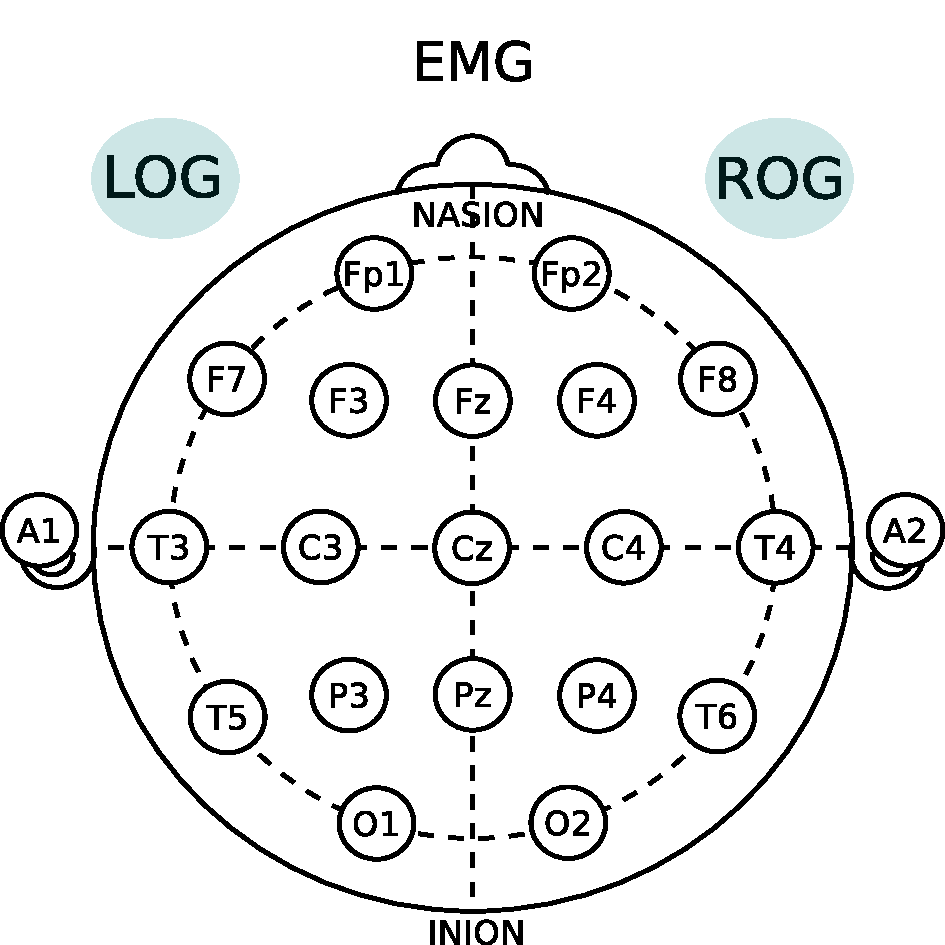
\includegraphics[width=0.15\textwidth]{./img_diagramas/cabecita_JGZ.pdf} \\
CLO & RLO & RRU & JGZ
\end{tabular}
\\
\begin{tabular}{ccc}
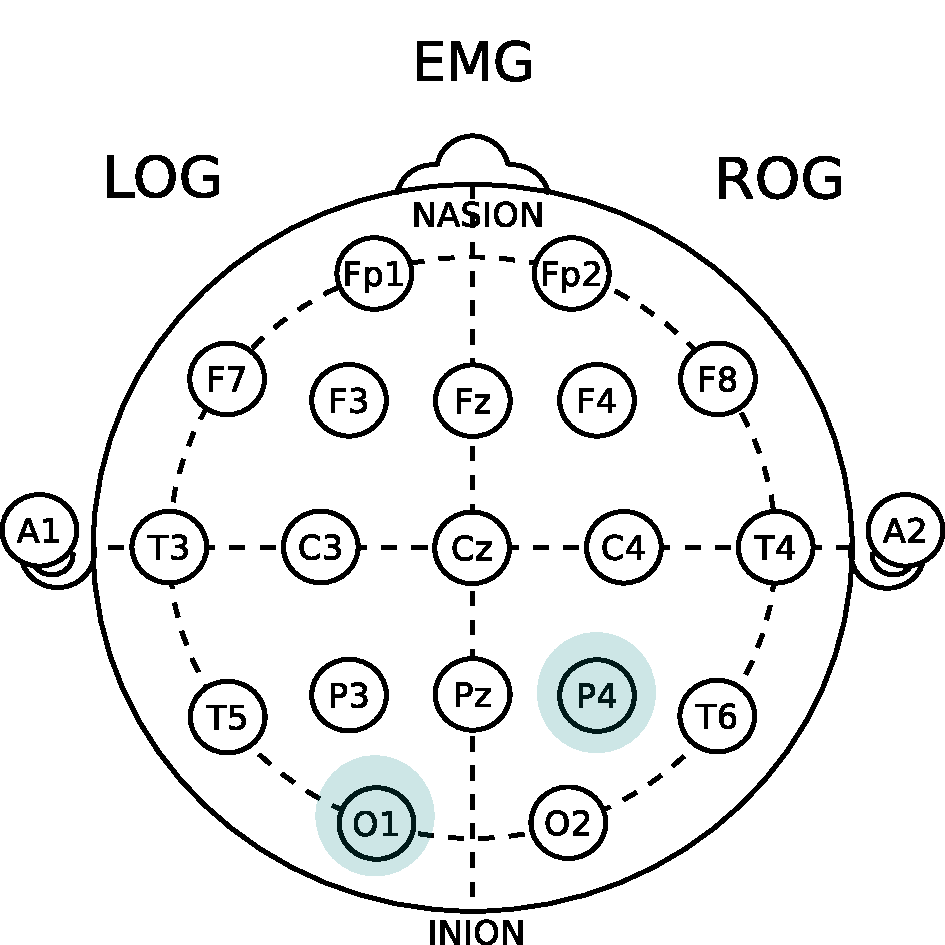
\includegraphics[width=0.15\textwidth]{./img_diagramas/cabecita_FGH.pdf} &
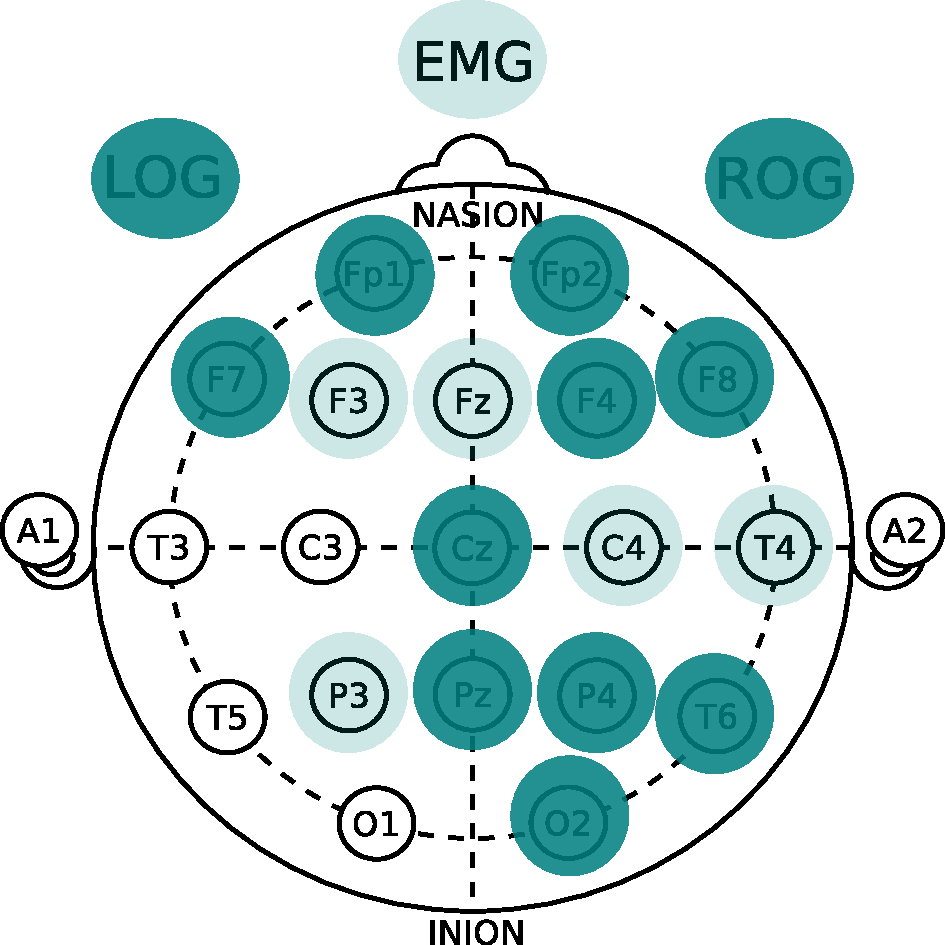
\includegraphics[width=0.15\textwidth]{./img_diagramas/cabecita_MGG.pdf} &
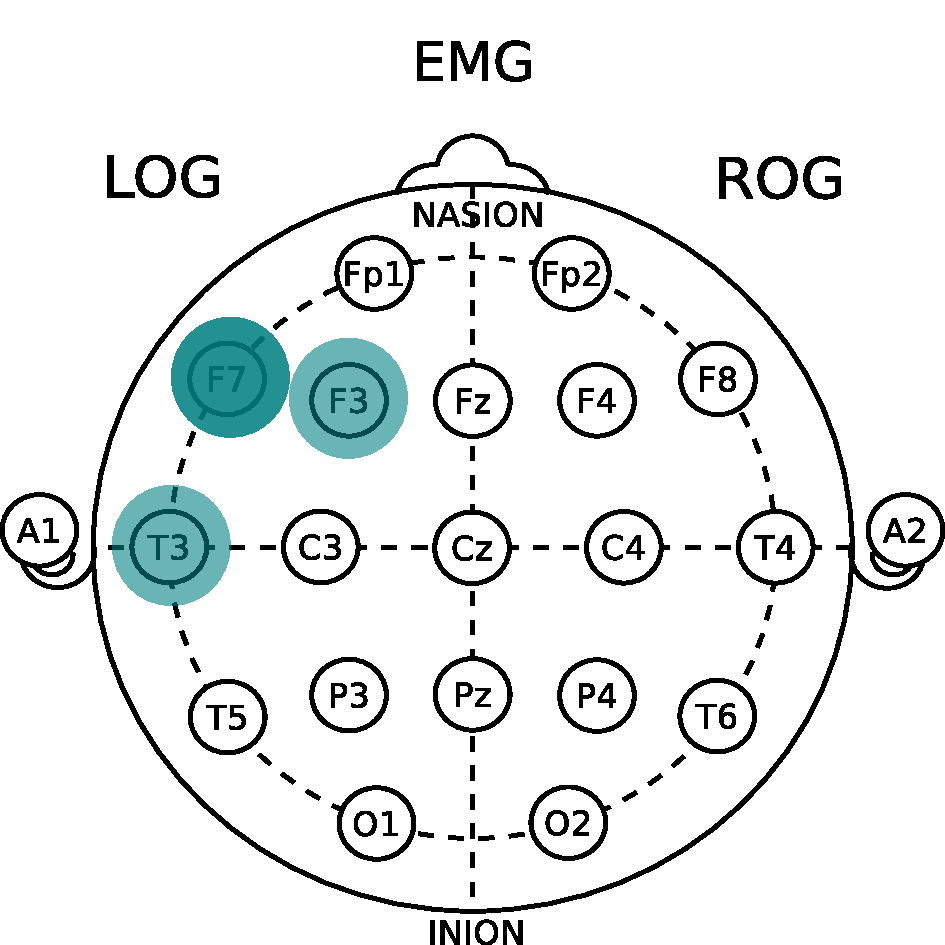
\includegraphics[width=0.15\textwidth]{./img_diagramas/cabecita_EMT.pdf} \\
FGH & MGG & EMT
\end{tabular}
\end{tabular}
\caption{Regiones donde se encontraron diferencias significativas al comparar las proporciones de 
épocas estacionarias durante sueño MOR y NMOR}
\label{cabecitas_munchas}
\end{figure}

Para corroborar la consistencia de las diferencias en LOG y ROG, se repitió la comparación a nivel 
grupal usando la prueba $U$ de  Mann-Whitney\footnote{Implementada en R como \texttt{wilcox.test}}
y se encontraron diferencias significativas ($p<0.05$) para el grupo Nn en los canales C4, F7, FP1, 
FP2, LOG y ROG, mientras que en el grupo Mn sólo se observaron tales diferencias en FP1, LOG y ROG 
(ver figura \ref{comparacion_verde});
las diferencias en la región frontal podrían ser fisiológicamente relevantes, ya que típicamente se 
asocia a la corteza frontal con la toma de decisiones.

El que se encontraran diferencias significativas para el grupo Nn, pero que no se encontraron en el
grupo Mn, sugiere que éstas pueden estar asociadas con el deterioro cognitivo.
Para probar tal hipótesis se comparó grupalmente la proporción de épocas estacionarias, tanto en
sueño MOR como NMOR (ver figura \ref{comparacion_graf}); no se encontraron diferencias
significativas ($p<0.05$).

\begin{figure}
\centering
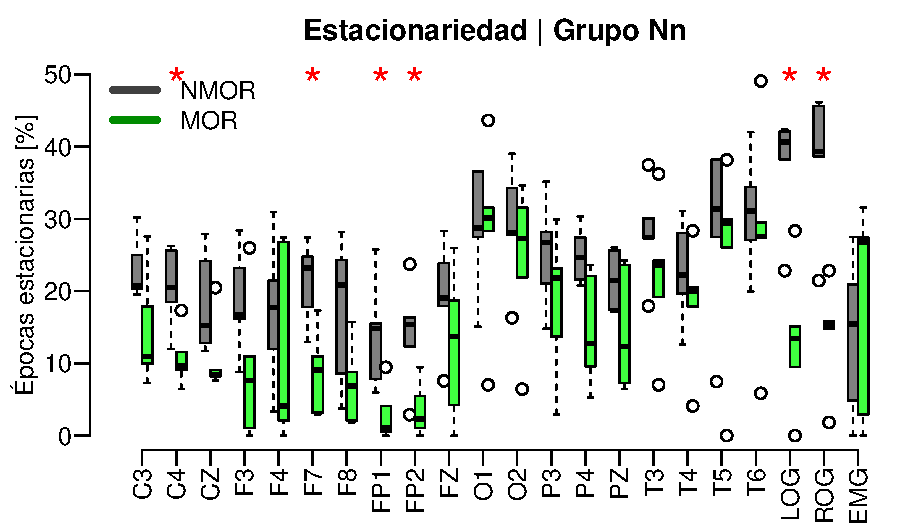
\includegraphics[width=\linewidth]
{./img_ejemplos/Comparacion_etapas_normal_MOR_vs_NMOR_v2.pdf} \\
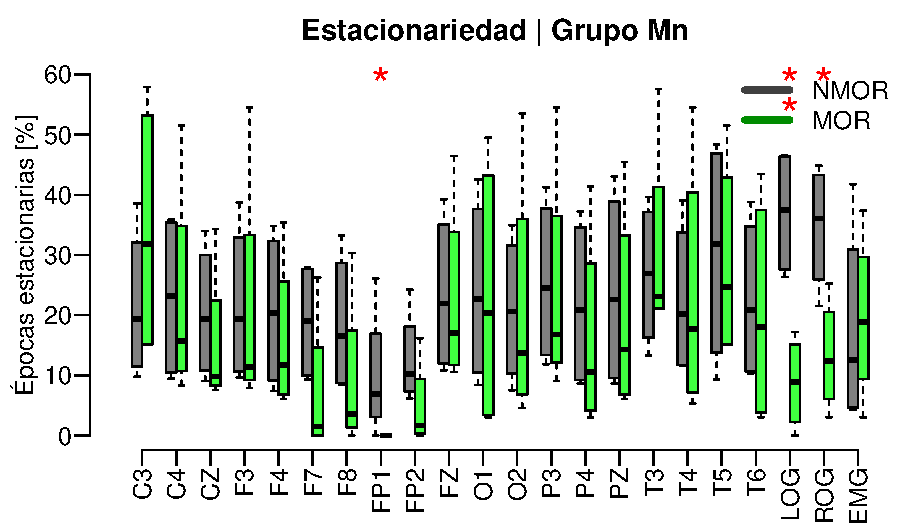
\includegraphics[width=\linewidth]
{./img_ejemplos/Comparacion_etapas_pdc_MOR_vs_NMOR_v2.pdf} \\
\caption{Comparación sobre las proporciones de épocas estacionarias durante sueño MOR y NMOR, para 
ambos grupos}
\label{comparacion_verde}
\end{figure}

\begin{figure}
\centering
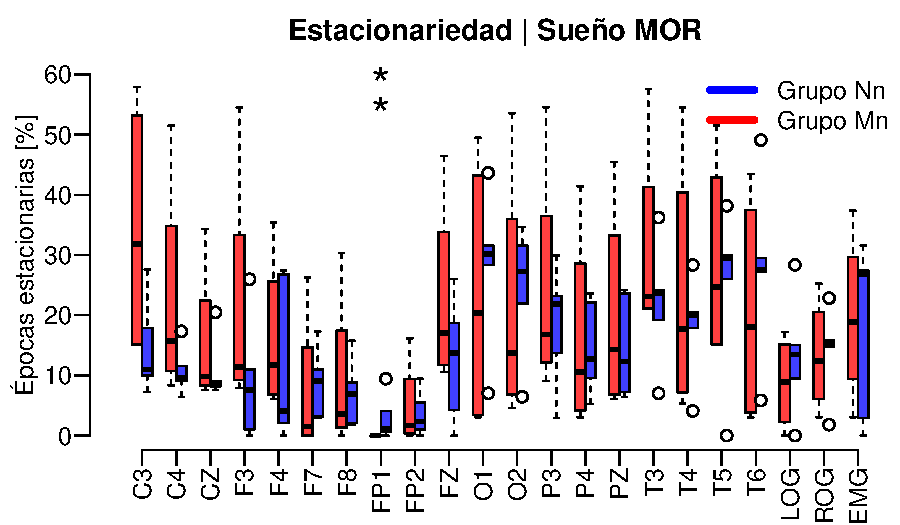
\includegraphics[width=\linewidth]
{./img_ejemplos/Comparacion_gpos_MOR_v2.pdf} \\
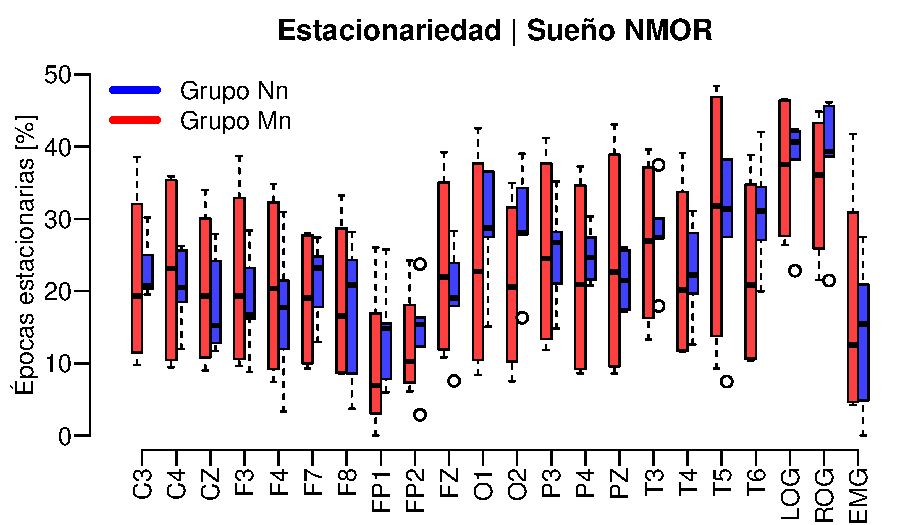
\includegraphics[width=\linewidth]
{./img_ejemplos/Comparacion_gpos_NMOR_v2.pdf}
\caption{Comparación sobre las proporciones de épocas estacionarias entre los grupos Nn y Mn, 
durante sueño MOR y NMOR}
\label{comparacion_graf}
\end{figure}

%%%%%%%%%%%%%%%%%%%%%%%%%%%%%%%%%%%%%%%%%%%%%%%%%%%%%%%%%%%%%%%%%%%%%%%%%%%%%%%%%%%%%%%%%%%%%%%%%%%
%%%%%%%%%%%%%%%%%%%%%%%%%%%%%%%%%%%%%%%%%%%%%%%%%%%%%%%%%%%%%%%%%%%%%%%%%%%%%%%%%%%%%%%%%%%%%%%%%%%

\section{Patrones visuales}

Los resultados anteriores, aparentemente contradictorios, indican que la comparación directa no es 
una herramienta efectiva para entender los cambios que se esperan en la estacionariedad durante
sueño MOR.
Como auxiliar visual, se \textit{graficaron} en el tiempo las épocas
estacionarias indicando por cada canal la porción del registro que se comporta como débilmente 
estacionario, como en la figura \ref{patroncito}.

%\begin{figure}
%\includegraphics[width=\textwidth]
%{./img_ejemplos/MJNNVIGILOS_est.png}
%\caption{Disposición gráfica para los resultados de la prueba PSR en el sujeto MJH. Se han 
%resaltado con color verde las épocas clasificadas como de sueño MOR.}
%\label{ejemplo_graf}
%\end{figure}

Al construir estos gráficos, se hacen visibles \textit{bloques} de épocas con propiedades 
similares; ha parecido conveniente investigar este fenómeno porque su estructura es independiente 
de los métodos planteados. En principio, la aparición de estos bloques es consistente con la
caracterización del sueño por etapas; por ejemplo,
estos bloques aparecen relacionados con la aparición de sueño MOR en todos los 
sujetos del grupo Mn bajo el siguiente patrón:
\begin{itemize}
\item Bloque abundante en épocas estacionarias, visualmente oscuro
\item Bloque abundante en épocas no-estacionarias, visualmente claro
\item Sección que contiene el sueño MOR
\end{itemize}

\begin{figure}
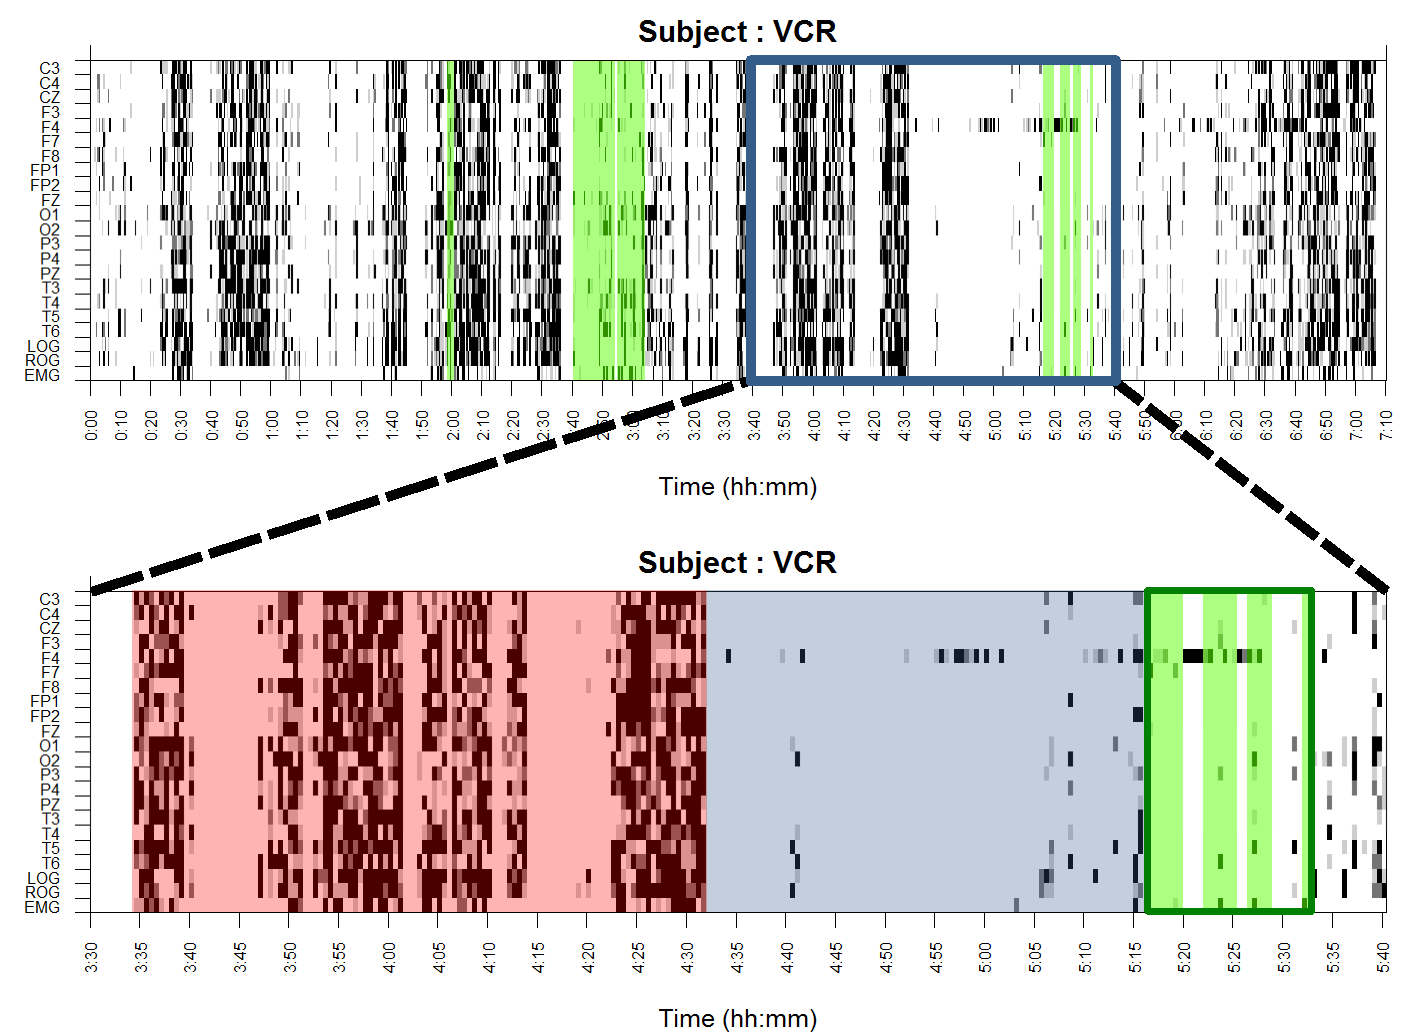
\includegraphics[width=\textwidth]
{./img_ejemplos/zoom_VCR.pdf}
\caption{Patrón propuesto como asociado con el sueño MOR: épocas estacionarias 
(rojo), épocas no-estacionarias (azul), bloque que contiene al sueño MOR}
\label{patroncito}
\end{figure}

Debido a que estos \textit{patrones de estacionariedad} se basan primeramente en propiedades del
espectro de potencias, se graficó el mismo para poder compararlos. Se encontró que, visualmente,
los patrones en la estacionariedad están relacionados con las ondas Beta.

El hecho que estos patrones se encuentren definidos vagamente ha dificultado su análisis, motivo
por el cual su estudio es limitado y se pretende como trabajo futuro.

%%%%%%%%%%%%%%%%%%%%%%%%%%%%%%%%%%%%%%%%%%%%%%%%%%%%%%%%%%%%%%%%%%%%%%%%%%%%%%%%%%%%%%%%%%%%%%%%%%%
%%%%%%%%%%%%%%%%%%%%%%%%%%%%%%%%%%%%%%%%%%%%%%%%%%%%%%%%%%%%%%%%%%%%%%%%%%%%%%%%%%%%%%%%%%%%%%%%%%%
%%%%%%%%%%%%%%%%%%%%%%%%%%%%%%%%%%%%%%%%%%%%%%%%%%%%%%%%%%%%%%%%%%%%%%%%%%%%%%%%%%%%%%%%%%%%%%%%%%%
%%%%%%%%%%%%%%%%%%%%%%%%%%%%%%%%%%%%%%%%%%%%%%%%%%%%%%%%%%%%%%%%%%%%%%%%%%%%%%%%%%%%%%%%%%%%%%%%%%%

\section{Discusión}

Este trabajo parte de la hipótesis de que adultos mayores con PDC presentan en mayor medida 
estacionariedad débil en sus registros de PSG; al comparar sujetos de los grupo Nn (control) y Mn 
(PDC), no se observaron cambios significativos en la porción de tiempo durante la cual el registro 
de PSG se comporta como débilmente estacionario. 
Esto puede interpretarse como que los cambios en la corteza cerebral durante el deterioro 
cognitivo, no provocan que  la señal se vuelva más \textit{simple} en el sentido de 
\textit{volverse} estacionaria.

Comparando grupalmente la cantidad de épocas estacionarias durante MOR y NMOR, se encontró que en 
el grupo Nn había diferencias significativas en sitios de la región frontal y que no eran presentes
en el grupo Mn; para poder establecer una relación con el PDC haría falta un mayor grupo muestral, 
o bien nuevos registros de PSG para los mismos sujetos, o incluso analizar registros de EEG durante 
otro tipo de actividades y confirmar las diferencias encontradas.

Cabe destacar que la evidencia aportada indica que el PSG es un conjunto de señales que se comportan
como no-estacionarias durante la mayor parte del sueño, lo cual confirma el supuesto usual de que 
las señales de origen biológico son por naturaleza no-estacionarias. 

\subsection{Efecto del tamaño de las época}

Como se mencionó anteriormente, el uso de épocas de 30 segundos está motivado por las 
recomendaciones de la AASM para clasificar, de manera estandarizada, las etapas de sueño en
registros de PSG \cite{AASM07}. 
%No se discutirán en este trabajo motivaciones o evidencia para usar esta longitud de época en 
%particular, ni para el caso contrario, sino que se acepta por fines de comparabilidad. 
Debido a un error técnico, en una etapa temprana de este trabajo se usaron épocas de 10 segundos 
para algunos análisis, una inconsistencia que eventualmente fue corregida.
Al efectuar los análisis descritos con otro tamaño de época, se produjeron resultados que distan
bastante de los finales, razón por la cual pareció conveniente investigar más este fenómeno.

En el apéndice X se explica que si disminuye el tamaño de época el test de PSR disminuye su 
potencia, de modo que es más propensa a dar falsos negativos (rechazar la hipótesis de 
estacionariedad cuando debía aceptarse); entonces, en épocas más pequeñas debería haber más épocas 
clasificadas como no-estacionarias.
Sin embargo, al \textit{graficar} la estacionariedad para diferentes tamaños de época (figura
\ref{comp_VCR}) ocurre que es más frecuente el efecto contrario.

\begin{figure}
\centering
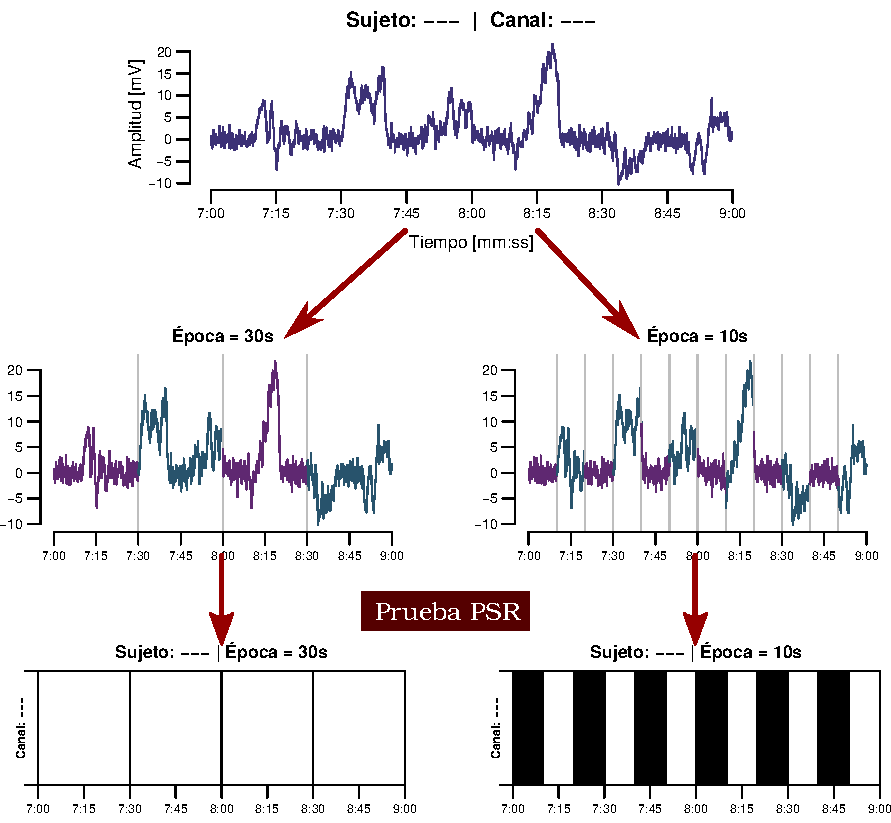
\includegraphics[width=\linewidth]{./img_diagramas/epocas_diferentes_v2.pdf}
\caption{Esquema de cómo se tomaron diferentes tamaños de época para estudiar los registros de 
PSG}
\label{epocas_diferentes}
\end{figure}

Se propone que este efecto puede ser explicado si los registros de PSG son \textbf{localmente
estacionarios}, una propiedad introducida por Dahlhaus \cite{Dahlhaus97} y que consiste en que un
proceso no-estacionario pueda ser aproximado a trozos \textit{ensamblando} procesos estacionarios
definidos para intervalos pequeños de tiempo.
Esta caracterización del EEG ha sido usada anteriormente de manera fructífera pero problemática
[??].

En el contexto particular del presente trabajo, la presencia de estacionariedad local puede ser
explicada fisiológicamente por el contenido heterogéneo de ritmos cerebrales de las etapas de 
sueño; como ejemplo, en la etapa N3 aparecen husos de sueño mezcladas con ritmos Alfa, de modo
que es posible hallar un fragmento de época en sueño N3 con únicamente un tren de ondas Alfa
o un tren de husos de sueño.
Este fenómeno es ilustrado de manera esquemática en la figura \ref{epocas_diferentes}.

\begin{figure}
\centering
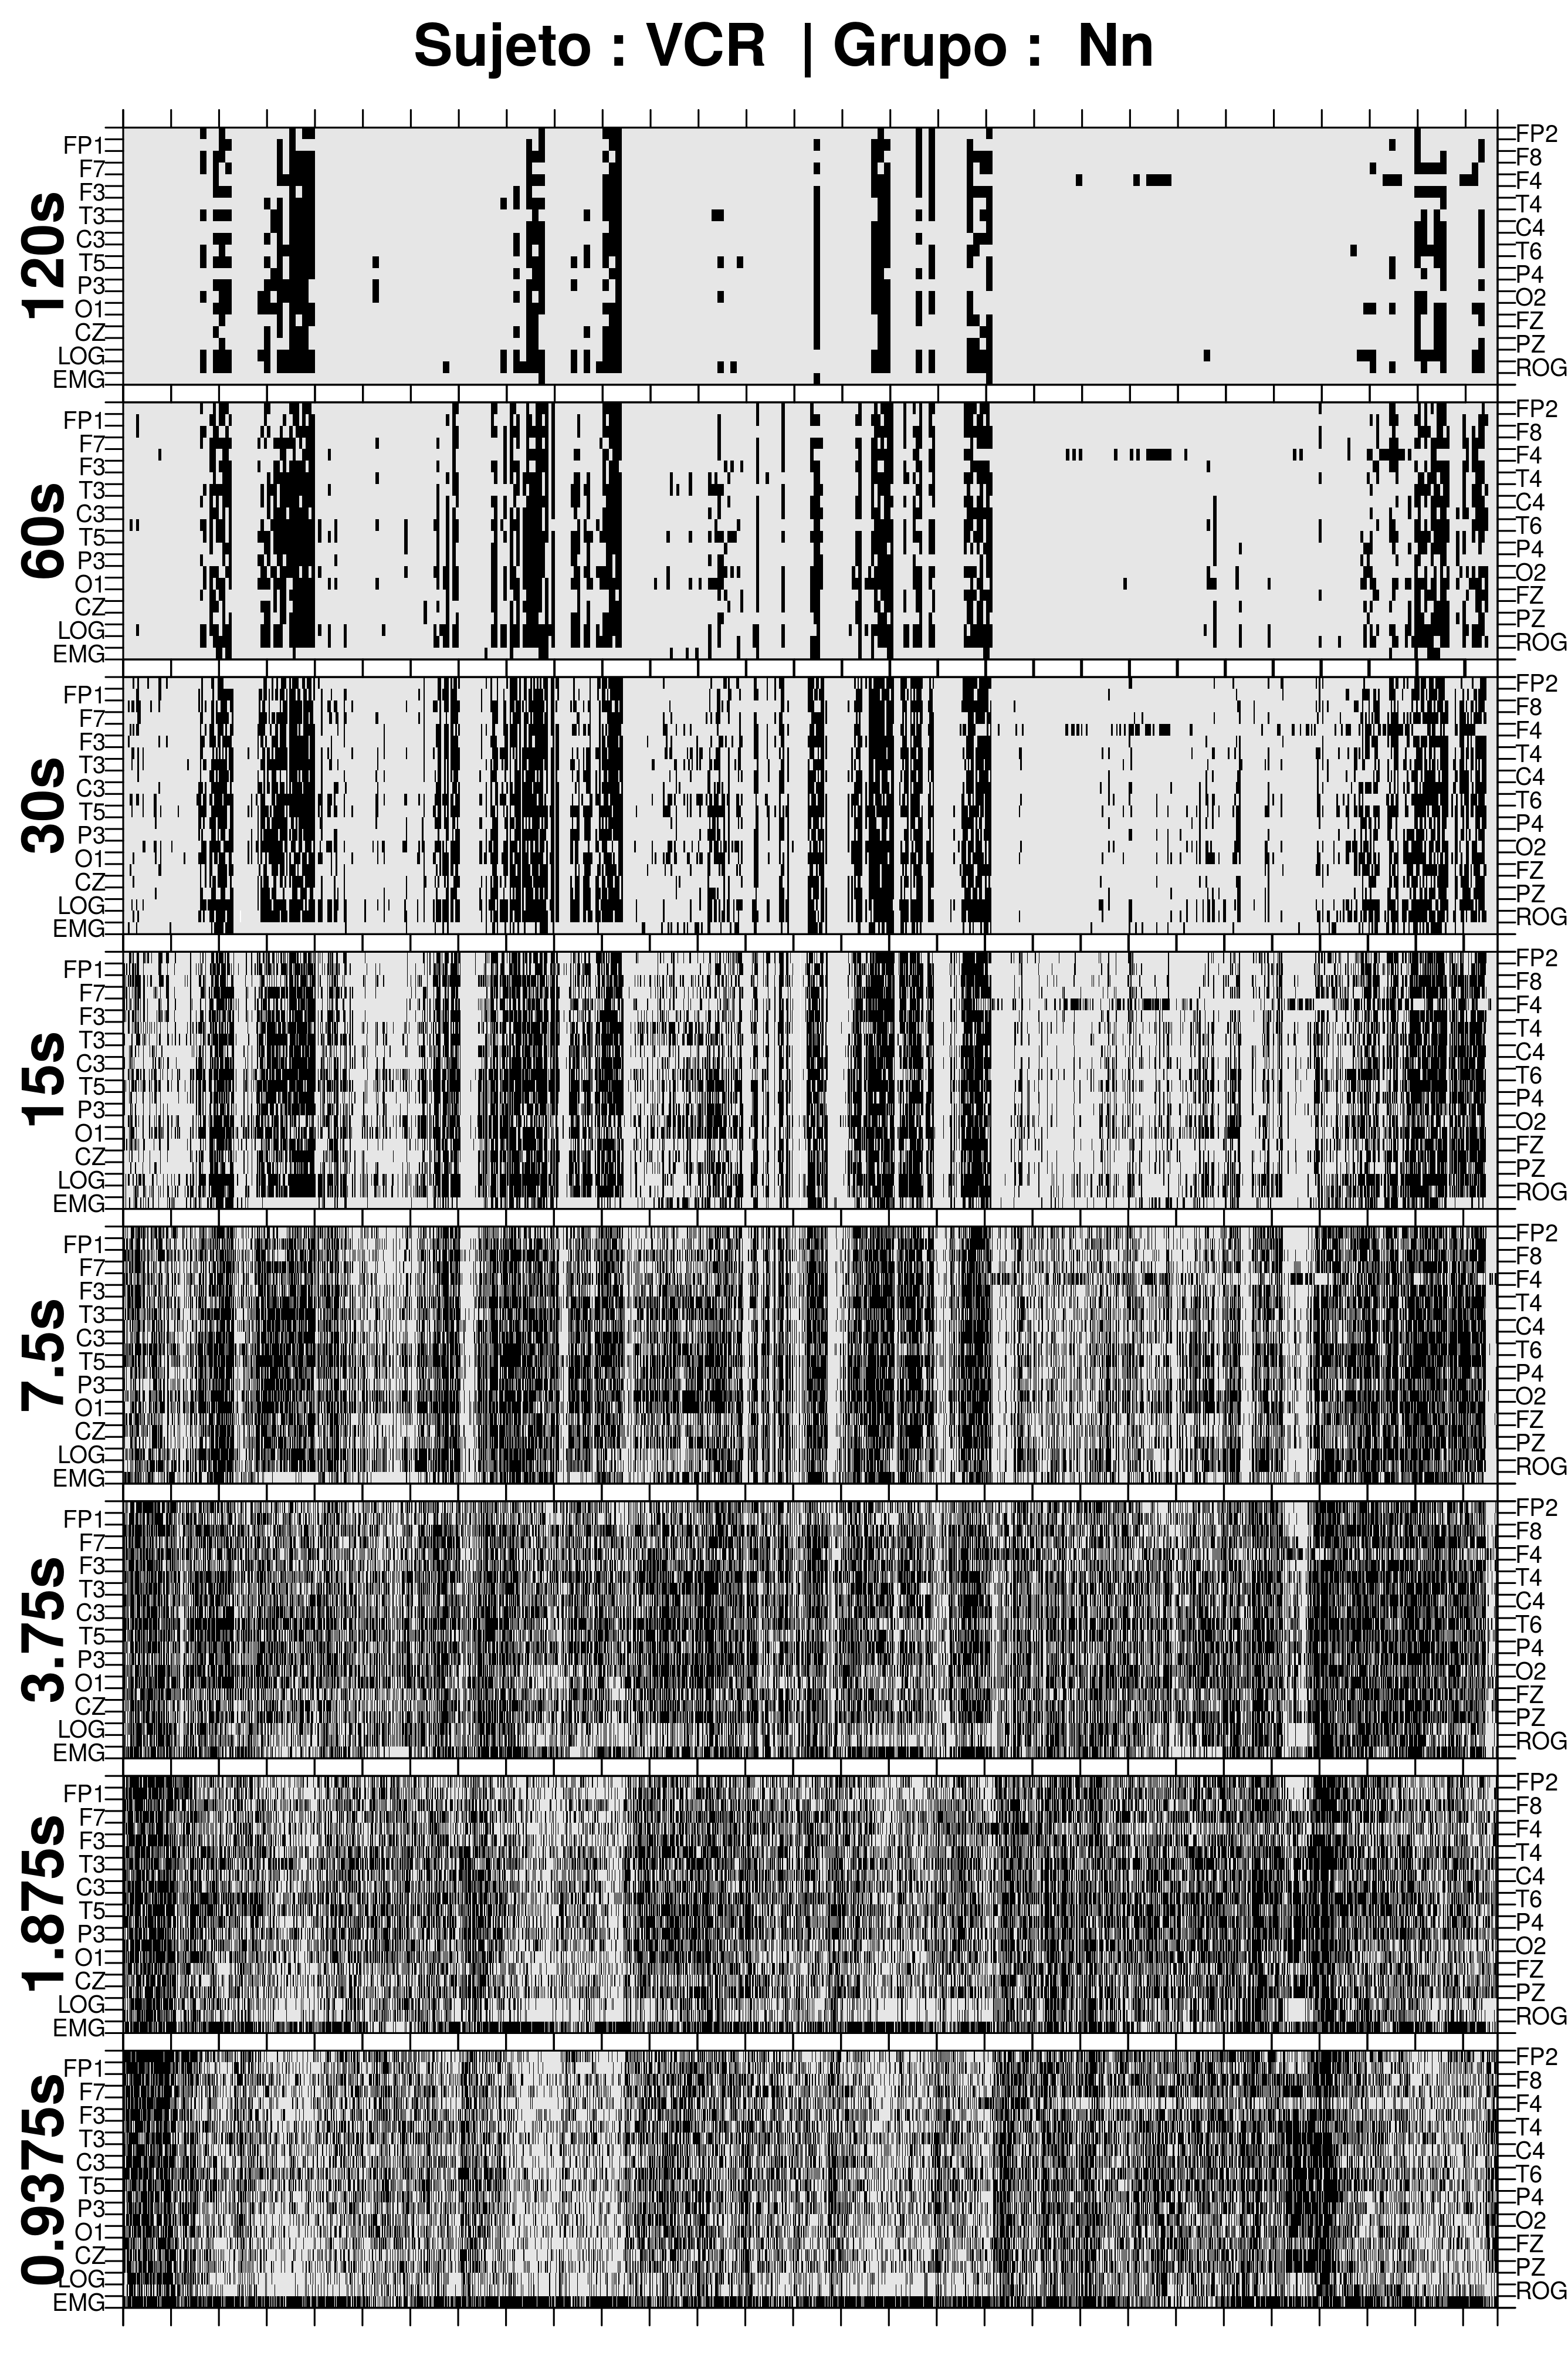
\includegraphics[width=0.7\linewidth]
{./img_ejemplos/VCNNS1_comp_est_.png}
\caption{Compilación gráfica de las épocas clasificadas como PE, distribuidas en el tiempo
para cada uno de los canales. El registro corresponde al sujeto VCR, organizando el registro en
épocas de diferente duración}
\label{comp_VCR}
\end{figure}

Entonces, se propone que los registros de PSG se comportan como procesos localmente estacionarios; 
más aún, se propone que esta característica cambia cualitativamente en adultos mayores con PDC,
para los cuales el \textit{nivel de homogeneidad} del PSG es muy similar durante MOR y NMOR.

%%%%%%%%%%%%%%%%%%%%%%%%%%%%%%%%%%%%%%%%%%%%%%%%%%%%%%%%%%%%%%%%%%%%%%%%%%%%%%%%%%%%%%%%%%%%%%%%%%%
%%%%%%%%%%%%%%%%%%%%%%%%%%%%%%%%%%%%%%%%%%%%%%%%%%%%%%%%%%%%%%%%%%%%%%%%%%%%%%%%%%%%%%%%%%%%%%%%%%%

%\subsection{Sobre los sujetos excluidos}
%
%Durante el trabajo se mencionan tres sujetos (FGH, MGG, EMT) cuyos registros de PSG fueron 
%analizados pero que no son considerados estadísticamente; cada uno de ellos fue excluido, por 
%diversos motivos, del trabajo por Vázquez Tagle y colaboradores \cite{VazquezTagle16}, pero 
%dieron su consentimiento informado para el registro de PSG, debido a lo cual analizó el efecto de 
%su inclusión dentro de los análisis.
%Destaca el sujeto FGH, quien padece de parálisis facial, cataratas, y problemas no especificados 
%en hipotiroides y columna; según se reporta, el sujeto no informó de estos últimos 
%padecimientos sino hasta después del registro de PSG, por lo que su exclusión se efectuó a 
%posteriori.
%
%Un vistazo a los registros 'inusuales' de FGH (figura\ref{FGH_psg}, comparar con 
%\ref{ejemplos_mor}) pudiera haber advertido que en el registro no hay actividad cerebral en los 
%canales correspondientes a la región izquierda (aquella con parálisis) sino ruido amplificado 
%del polisomnógrafo.
%Dentro del marco de este trabajo, destacan las proporciones inusuales de épocas PE (cercanas a 1 
%o 0) para este sujeto en los canales F4, F7, F8, FP1, FP2, FZ, tanto en sueño MOR como NMOR; 
%usando la representación gráfica para FGH, es visible una inusual ausencia total de 
%estacionariedad en tales canales (figura \ref{FGH_especial}, comparar con \ref{ejemplo_graf}). 
%Si bien esta metodología no se diseñó para tal fin, aún así se pudo detectar la falta de 
%actividad cerebral.
%
%\begin{figure}
%\centering
%\includegraphics[width=0.95\linewidth]
%{./img_ejemplos/FGH_297_PDG_lucirse_PSG.pdf} 
%\caption{Una época típica del registro PSG para el sujeto FGH durante sueño MOR. Nótense 
%los patrones periódicos en los canales correspondientes a la región frontal, que no 
%corresponden a la actividad cerebral usual.}
%\label{FGH_psg}
%\end{figure}
%
%\begin{figure}
%\centering
%\includegraphics[width=0.95\linewidth]
%{./img_ejemplos/FGHSUE_est.png} 
%\caption{Compilado gráfico para el sujeto FGH; nótese el patrón inusual (completamente 
%blanco o negro) en los canales correspondientes a la región frontal}
%\label{FGH_especial}
%\end{figure}

%%%%%%%%%%%%%%%%%%%%%%%%%%%%%%%%%%%%%%%%%%%%%%%%%%%%%%%%%%%%%%%%%%%%%%%%%%%%%%%%%%%%%%%%%%%%%%%%%%%
%%%%%%%%%%%%%%%%%%%%%%%%%%%%%%%%%%%%%%%%%%%%%%%%%%%%%%%%%%%%%%%%%%%%%%%%%%%%%%%%%%%%%%%%%%%%%%%%%%%

%%%%%%%%%%%%%%%%%%%%%%%%%%%%%%%%%%%%%%%%%%%%%%%%%%%%%%%%%%%%%%%%%%%%%%%%%%%%%%%%%%%%%%%%%%%%%%%%%%%
%%%%%%%%%%%%%%%%%%%%%%%%%%%%%%%%%%%%%%%%%%%%%%%%%%%%%%%%%%%%%%%%%%%%%%%%%%%%%%%%%%%%%%%%%%%%%%%%%%%

\section{Conclusiones}

En registros de PSG para adultos mayores, segmentados en épocas de 30 segundos, la presencia 
proporcional de estacionariedad débil es significativamente diferente ($p<0.05$) durante el sueño 
MOR y NMOR;
Estas diferencia fueron presentes para el grupo Mn en los canales C4, F7, FP1, FP2, LOG, ROG, y 
para el grupo Mn en los canales LOG y ROG.
Estas diferencias pueden explicarse 
(1) en LOG y ROG por las características del sueño MOR y
(2) en los canales C4, F7, FP1, FP2, por tratarse del lóbulo frontal, típicamente asociado con la 
toma de decisiones.

%El análisis de estacionariedad sobre registros de PSG para un adulto mayor con parálisis facial 
%fue capaz de señalar este padecimiento, visto como una ausencia total de épocas estacionarias
%en una región concreta.

Estos resultados sugieren que el método de comparación es sensible a los cambios funcionales del 
cerebro al transitar entre etapas de sueño; tales cambios son menos \textit{visibles} en presencia
de PDC. Esta interpretación propuesta es consistente con \cite{Valeria}.

%En otro ámbito, los patrones visuales descritos, visibles al mostrar gráficamente la 
%distribución de épocas PE, predicen parcialmente con las épocas de sueño MOR clasificadas 
%por un experto (cuando menos en el grupo Control).
%Se propone que la representación gráfica pudiera ser usado como auxiliar en la clasificación 
%de segmentos de registro según la etapa de sueño.

Los datos recabados son evidencia que los registros de PSG en adultos mayores no pueden 
considerarse en general como series de tiempo estacionarias o no-estacionarias, sino que sus 
propiedades estadísticas cambian en el tiempo conforme se transita entre diferentes estados 
fisiológicos; 
%esta característica no puede ser ignoradaal modelar este tipo de señales.
esta característica ha sido considerada anteriormente \cite{Kaiser00}, pero usualmente es ignorada
en base al diseño experimental.

%%%%%%%%%%%%%%%%%%%%%%%%%%%%%%%%%%%%%%%%%%%%%%%%%%%%%%%%%%%%%%%%%%%%%%%%%%%%%%%%%%%%%%%%%%%%%%%%%%%
%%%%%%%%%%%%%%%%%%%%%%%%%%%%%%%%%%%%%%%%%%%%%%%%%%%%%%%%%%%%%%%%%%%%%%%%%%%%%%%%%%%%%%%%%%%%%%%%%%%

\section{Trabajo a futuro}

%Los resultados principales de este trabajo, con vista al trabajo futuro, consiste en las 
%diferencias encontradas entre el sueño MOR y NMOR, así como los patrones visuales asociados con 
%la aparición de sueño MOR; tales características sólo fueron presentes para el grupo 
%Control. Si bien no constituyen propiamente marcadores de deterioro cognitivo, esta metodología
%podría extenderse para identificar tales marcadores.
%Por ejemplo, un marcador conocido \cite{Becerra12} del deterioro cognitivo es el 'enlentecimiento' 
%de la actividad cerebral, entendido como un cambio en la concentración de energía desde ondas 
%rápidas a ondas lentas.
%Para detectar la estacionariedad débil se ha usado prueba de Priestley-Subba Rao, basada en 
%estimadores locales para la función de densidad espectral (FDE); estos mismos estimadores 
%podrían ser usados para corroborar si efectivamente existen diferencias en la FDE para registros 
%de adultos mayores con y sin deterioro cognitivo. 
%
%Finalmente, y como se mencionó anteriormente, los patrones visuales en la representación 
%gráfica pueden tener un uso como características auxiliares para la detección 
%semi-automática de épocas MOR en registros de PSG; en ese sentido, cabe mencionar el caso de 
%los sujetos excluidos del estudio, para los cuales estos patrones parecen no cumplirse. 
%Es en principio posible que la identificabilidad del sueño MOR, a través de estos patrones, 
%pudiera fungir como marcador clínico.

%%%%%%%%%%%%%%%%%%%%%%%%%%%%%%%%%%%%%%%%%%%%%%%%%%%%%%%%%%%%%%%%%%%%%%%%%%%%%%%%%%%%%%%%%%%%%%%%%%%
%%%%%%%%%%%%%%%%%%%%%%%%%%%%%%%%%%%%%%%%%%%%%%%%%%%%%%%%%%%%%%%%%%%%%%%%%%%%%%%%%%%%%%%%%%%%%%%%%%%
%%%%%%%%%%%%%%%%%%%%%%%%%%%%%%%%%%%%%%%%%%%%%%%%%%%%%%%%%%%%%%%%%%%%%%%%%%%%%%%%%%%%%%%%%%%%%%%%%%%
%%%%%%%%%%%%%%%%%%%%%%%%%%%%%%%%%%%%%%%%%%%%%%%%%%%%%%%%%%%%%%%%%%%%%%%%%%%%%%%%%%%%%%%%%%%%%%%%%%%
